
\PassOptionsToPackage{rgb,table}{xcolor}

% Activate if you want to compile slides.
\documentclass{beamer}

% Activate if you want to compile handout.
%\documentclass[handout]{beamer}

\usetheme{default}

%% TeX Settings
\input{packages.tex}
\input{colors.tex}
\usepackage{tabularx}
\usepackage{hyperref}

%% Meta Data and Variables
\input{meta.tex}
\title{Vergleich Constant Function Market Maker}

%% Presentation Style Settings
\input{style.tex}
\input{titlepage.tex}

%% Document
\begin{document}
  \begin{frame}[plain]
    \titlepage
  \end{frame}
  
\begin{frame}{Übersicht}{Aufbau der Präsentation}
  \tableofcontents
\end{frame}

\section{Einführung}

\subsection{Krypto-Tauschbörsen}

\begin{frame}{Krypto-Tauschbörsen}{eine Übersicht}

\begin{figure}[h!]
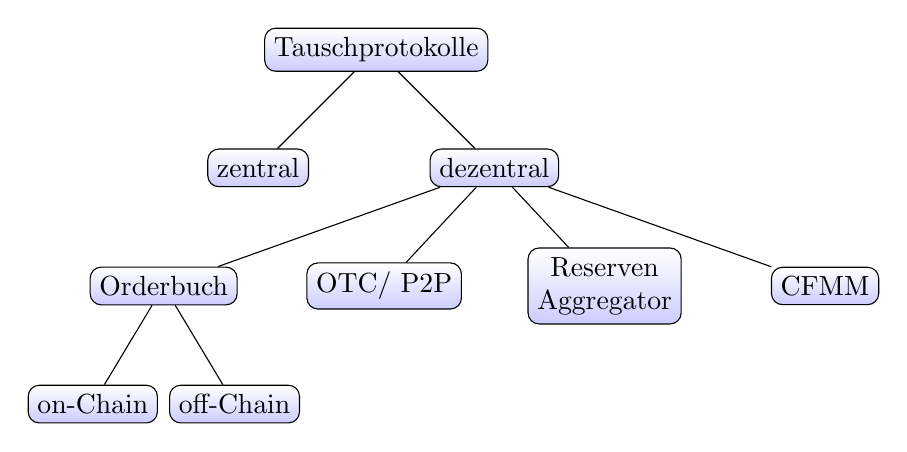
\begin{tikzpicture}
[ sibling distance =10em ,
every node/.style = {shape=rectangle, rounded corners,
	draw , align = center ,
	top color=white, bottom color = blue!20}]]
 \tikzstyle{level 1}=[sibling distance=30mm]
 \tikzstyle{level 2}=[sibling distance=28mm]
 \tikzstyle{level 3}=[sibling distance=18mm]
  
  \node {Tauschprotokolle}
  	child { node {zentral}}
  	child { node {dezentral}
  		child { node {Orderbuch}
  			child { node {on-Chain}}
  			child { node {off-Chain}}}
  		child { node {OTC/ P2P}}
  		child { node {Reserven \\Aggregator}}
  		child { node {CFMM}}
  		};
\end{tikzpicture}
\caption{\tiny{Quelle: eigene Darstellung in Anlehnung an Schär (2020, S.8-11)}}
\end{figure}
\end{frame}

\subsection{Constant Function Market Makers}

\begin{frame}{Constant Function Market Maker}{Eigenschaften}
  \begin{enumerate}
    \item<1->{Smart Contract basierte Liquiditätspools: halten Reserven von 2 oder mehr Kryptoassets}
    \item<2->{von einem Code kontrolliert}
    \item<3->{Code führt eine Funktion aus}
    \item<4->{kein Orderbuch: Nutzer handeln direkt gegen den Kontrakt}
    \item<5->{ökonomische Anreize für Liquiditätsprovider}
    \end{enumerate}
\end{frame}

\begin{frame}{Constant Function Market Maker}{Vorteile}
  \begin{enumerate}
    \item<1->{kein Gegenparteirisiko: beide Seiten des Tauschs finden in einer einzelnen Blockchain-Transaktion statt}
    \item<2->{Zensurresistenz, keine Listungsgebühren, keine Spreads}
    \item<3->{Platzsparend: Status kann über Anzahl der gepoolten Assets eindeutig repräsentiert werden}
    \item<4->{Offenheit: interne Logik des Smart Contracts kann beobachtet werden, durch Blockchain besichert}
    \item<5->{Integration: Smart Contracts können in weitere Applikationen integriert werden}
    \item<6->{Liquidität: Funktionen stellen stetige Liquidität sicher und determinieren die Preise}
  \end{enumerate}
  \vspace{1em}
  \uncover<6->{
    Frage: Wie sehen diese Funktionen aus?
  }
\end{frame}


\begin{frame}{Constant Function Market Maker}{Protokolle}
	Antwort: Unterschiedlich! Gemeinsamkeit ist die Anwendung einer \textbf{konvexen} Funktion.
	\vspace{1em}
  \begin{itemize}
    \item{UniSwap} \includegraphics[width=0.5cm]{Uniswap Logo}
    \item{Balancer} \includegraphics[height=0.4cm]{Balancer Logo}
    \item{Curve} \includegraphics[width=0.4cm]{Curve Logo}
    \item{Bancor} \includegraphics[height=0.4cm]{Bancor Logo}
  \end{itemize}
   \vspace{1em}
    Vergleich: Funktionsgleichung, Slippage, Impermanent Loss und Liquiditätsbereitstellung
\end{frame}


\section{Protokollvergleich}


\subsection{UniSwap}

\begin{frame}{UniSwap}{allgemein}
 \begin{enumerate}
    \item<1->{ermöglicht automatischen Tausch zwischen ETH/ERC20-Token oder ERC20-/ERC20-Token}
    \item<2->{Preise werden über Constant Product Gleichung bestimmt}
    \item<3->{Gebühr von 0.3\%}
    \item<4->{Gebühr wird nach dem Tausch zum Liquiditätspool hinzugefügt}
  \end{enumerate}
\end{frame}

\begin{frame}{UniSwap}{Funktionsgleichung}
\begin{itemize}
\item{Constant Product Funktion:
    \begin{equation}
    x \cdot y = k
    \end{equation} }
\end{itemize}
\begin{figure}
\includegraphics[width=10cm]{Graphik CFMM}
\caption{\tiny{Quelle: Schär (2020, S.10)}}
\end{figure}
\end{frame}

\begin{frame}{UniSwap}{Tausch - Formeln und Beispiel}
\begin{itemize}
\item{Herleitung der Tausch-Formel:
	\begin{align*}
	k &= x\cdot y \\
	k &= (x+ (1-f)\Delta x) \cdot (y+\Delta y) \\
	\Delta y &= \dfrac{k}{x+ (1-f) \Delta x} - y \\
	\end{align*}}
\item{Beispiel: $x =10$,  $y=10$,  $f=0.003$ ,  $\Delta x = 1$ \\
	\begin{equation*}
	\dfrac{100}{10+(1-0.003)1}- 10 = -0.9066
	\end{equation*}}
 \item{Für das senden von 1 Einheit $x$ erhalten wir ca. 0.907 Einheiten $y$}
\end{itemize}
\end{frame}	

\begin{frame}{UniSwap}{effektiver Preis und Spot Preis}
\begin{itemize}
 \item<1->{Der effektive Preis für eine Einheit x-Token ist: $EP_{x} = \dfrac{\Delta y}{\Delta x}$}
 \item<2->{Somit gilt: $EP_{x}= 0.9066$ y-Token}
 \item<3->{Spot-Preis: marginaler Preis für einen Trade}
 \item<4->{über partielle Ableitung der Constant Product Gleichung}
 \item<5->{Spot-Preis von x: $SP_{x} = \dfrac{y}{x}$}
 \item<6->{$SP_{x}$ vor dem Trade:  $\dfrac{y}{x} = 10/10 = 1$}
 \item<7->{$SP_{x}$ nach dem Trade:  $\dfrac{y + \Delta y}{x + \Delta x} = \dfrac{10+(-0.9066)}{10+1} = 0.827$}
 \item<8->{Preis von $x$ hat durch den Trade abgenommen, alle Trades verändern den Spot-Preis}
\end{itemize}
\end{frame}

\begin{frame}{UniSwap}{Slippage}
\begin{itemize}
 \item<1->{Die Abweichung vom Spot-Preis zum effektiven Preis nennt sich Slippage}
 \item<2->{SL = $\dfrac{EP_{x}}{SP_{x}} - 1$ = $(0.9066 / 1) - 1$ = $ -0.0934 $}
 \item<3->{Der Slippage bei dem Trade ist somit ca. 9.34\%}
 \item<4->{Slippage ist abhängig von der Grösse des Trades im Verhältnis zur Grösse des Pools}
 \item<5->{kommt durch die Konvexität der Kurve zustande}
 \item<6->{Arbitrage-Möglichkeit, da relativer Preis im Pool nicht mehr dem Aussenmarkt entspricht}
\end{itemize}
\end{frame}

\begin{frame}{UniSwap}{Liquidität bereitstellen}
 \begin{itemize}
    \item<1->{initialer Liquiditätsprovider kann Token-Verhältnis beliebig festlegen}
    \item<2->{aber: wenn der relative Preis der Token nicht dem Aussenmarkt-Preis entspricht $\rightarrow$ Arbitrage}
    \item<3->{grundsätzlich Token im gleichen Wert bereitstellen}
    \item<4->{Liquiditätsprovider erhält Liquiditätstoken}
    \item<5->{Liquidität abziehen: Liquiditätstoken werden \glqq vernichtet\grqq , enthalten proportionalen Anteil gesammelter Tauschgebühren}
  \end{itemize}	
\end{frame}

\begin{frame}{UniSwap}{Impermanent Loss}
 \begin{itemize}
    \item<1->{\textbf{Definition:} Verlust der durch das Poolen der Assets entsteht, verglichen mit dem Halten der Assets}
    \begin{itemize}
    \item{wichtig: wird erst bei Abzug der Mittel realisiert und entsteht nur bei relativem Preisunterschied der Assets}
    \end{itemize}
   \vspace{1em}
    \item<2->{\textbf{Grund:} verändert sich der Preis eines Tokens auf dem Aussenmarkt $\rightarrow$ Arbitrage bis wieder dem Aussenmarkt entspricht
    $\rightarrow$ Veränderung der Token Reserven im Pool und somit Veränderung der Token bei Abzug}
  \end{itemize} 	
\end{frame}

\begin{frame}{UniSwap}{Impermanent Loss - Beispiel}
 \begin{enumerate}
    \item<1->{Ausgangslage: 10 x-Token und 10 y-Token, beide Token sind jeweils 1\$ Wert}
    \item<2->{Annahmen: Wir haben den ganzen Pool bereitgestellt, keine Tradegebühren}
    \item<3->{Preis von x-Token auf dem Aussenmarkt verdoppelt sich $\rightarrow$ Arbitrage}
    \item<4->{Über Kombination der Spot-Preis Formel mit der Constant Product Gleichung können wir die neuen Pool Reserven bestimmen}
    \item<5->${x=\sqrt{k/SP_{x}} = \sqrt{100/2} = 7.0716}$
    \item<6->${y=100/7.0716 = 14.142}$
    \item<7->{Pool Wert neu = $7.0716 \cdot 2\$ + 14.142 \cdot 1\$ = 28.284 \$ $}
    \item<8->{Haltewert neu = $ 10 \cdot 2\$ + 10 \cdot 1\$ = 30\$ $}
  \end{enumerate}	
\end{frame}

\begin{frame}{UniSwap}{Impermanent Loss}
 \begin{itemize}
    \item<1->{allgemeine Impermanent Loss-Formel: 
    \begin{equation*}
    IL = \dfrac{Pool Wert^{\$}_{neu}}{Haltewert^{\$}_{neu}}-1
    \end{equation*}
     }
    \item<2->{Impermanent Loss im Beispiel: (28.284 / 30) - 1 = -0.057}
    \item<3->{UniSwap IL in Abhängigkeit des Preisunterschieds:
    \begin{equation*}
    IL =\dfrac{2 \sqrt{\Delta P^{\$}_{x} \Delta P^{\$}_{y}}}{\Delta P^{\$}_{x}+\Delta P^{\$}_{y}}-1 
    \end{equation*}
     }
   \item<3->{wobei $\Delta P = \dfrac{Preis_{neu}}{Preis_{alt}}$}  
   \end{itemize}	
   \uncover<2->{
    Unsere Assets haben ca. 5.7\% weniger Wert, als wenn wir sie einfach gehalten hätten! \textbf{Aber:} konnten Gebühren sammeln.
  }
\end{frame}


\subsection{Balancer}

\begin{frame}{Balancer}{Funktionsgleichung}
\begin{itemize}
  \item<1->{Erweitert das Konzept von UniSwap auf Pools mit bis zu 8 verschiedenen Token}
  \item<1->{Constant Value Funktion
  \begin{equation}
  V = \prod_t B^{w_{t}}_{t}
  \end{equation}
  }
  \item<1->{$B_{t}$ Anzahl Token $t$}
  \item<1->{$w_{t}$ normalisiertes Gewicht von Token $t$}
  \item<2->{normalisiertes Gewicht entspricht dem Wertanteil von $t$ am gesamten Pool-Wert}
  \item<2->{Summe der normalisierten Gewichte ist 1}
  \item<2->{Gewicht und damit Wertanteil eines Tokens im Pool bleibt konstant}
\end{itemize}  
\end{frame}

\begin{frame}{Balancer}{Liquidität bereitstellen}
\begin{itemize}
\item<1->{alle Token mit entsprechender Gewichtung oder nur ein einziger Token}
\item<2->{Hinzufügen eines einzelnen Tokens A ist gleichzusetzen mit dem Hinzufügen aller Token und dem sofortigen Austausch der restlichen Token zu Token A}
\item<3->{daher: Einzel-Deposit mit Gebühr}
\end{itemize}
\end{frame}

\begin{frame}{Balancer}{Tausch-Formel, Spot-Preis und effektiver Preis}
\begin{itemize}
 \item{Tausch-Formel:
 \begin{equation*}
  A_{o} = B_{o} \cdot \Biggl(1-\biggl(\dfrac{B_{i}}{B_{i}+ A_{i}}\biggr)^{\tfrac{w_{i}}{w_{o}}}\Biggr)
 \end{equation*}
 }
 \item{effektiver Preis:
 \begin{equation*}
 EP_{i}=\dfrac{A_{o}}{A_{i}}
 \end{equation*}
 }
 \item{Spot-Preis:
 \begin{equation*}
 SP_{i} = \dfrac{\frac{B_{o}}{w_{o}}}{\frac{B_{i}}{w_{i}}}
 \end{equation*}
 }
\end{itemize}
\end{frame}

\begin{frame}{Balancer}{Slippage}
\begin{itemize}
\item<1->{Einsetzen von $EP_{i}$ und $SP_{i}$ in die bekannte Slippage Gleichung ergibt:
\begin{equation*}
	SL= \dfrac{A_{o}}{A_{i}} \cdot \dfrac{B_{i}}{B_{o}} \cdot \dfrac{w_{o}}{w_{i}} -1
\end{equation*}
}
\item<1->{Die Höhe des Slippage ist somit abhängig vom relativen Pool-Gewicht der beiden gehandelten Token}
\begin{itemize}
\item{Dazu in der Diskussion mehr}
\end{itemize}
\end{itemize}
\end{frame}

\begin{frame}{Balancer}{Impermanent Loss}
\begin{itemize}
 \item<1->{Gleichung wie zuvor, nun generalisiert für n-Token
 in Abhängigkeit des Preisunterschieds:
 \begin{equation*}
 IL = \dfrac{\prod_{t}(\Delta P^{\$}_{t})^{w_{t}}}{\sum_{t}(\Delta P^{\$}_{t} \cdot w_{t})}-1
 \end{equation*}
 }
 \item<2->{Impermanent Loss ist somit auch von Gewichten abhängig}
 \begin{itemize}
\item{Ebenfalls in der Diskussion mehr}
 \end{itemize}
\end{itemize}
\end{frame}

\subsection{Curve}

\begin{frame}{Curve}{allgemein}
\begin{itemize}
 \item<1->{Tausch zwischen Stablecoins}
 \item<2->{Hintergrund: Slippage für Trade von Assets, die preisstabil bleiben sollten, nicht wünschenswert}
 \item<3->{Kombination von Constant Sum- und Constant Product-Function}
 \item<4->{Hybrid Constant Function Market Maker}
\end{itemize}
\end{frame}

\begin{frame}{Curve}{Funktionsgleichung}
\begin{itemize}
 \item{Curve Funktion:
 \begin{equation}
 An^n\sum x_{i}+D = ADn^n + \dfrac{D^{n+1}}{n^{n} \prod x_{i}}
 \end{equation}
 }
\end{itemize}
\begin{figure}
\includegraphics[width=8cm]{Graphik Curve} \caption{\tiny{Quelle: Egorov (2019, S.3)}}
\end{figure} 
\end{frame}

\begin{frame}{Curve}{Slippage}
\begin{itemize}
 %\item{Constant Sum: $\sum x_{i}= D$}
 %\item{Constant Product für Token mit gleichen Preisen: $\prod x_{i} = \biggl(\dfrac{D}{n}\biggr)^n$}
 \item{Kurve bei Pool-Gleichgewicht nur schwach gekrümmt}
 \item{Effektiver Preis weicht nur leicht vom Spot-Preis ab $\rightarrow$ tiefer Slippage}
 \item{ausserhalb des Gleichgewichts: Slippage, dafür immernoch Liquidität}
\end{itemize}
\end{frame}

\begin{frame}{Curve}{Liquidität bereitstellen und Impermanent Loss}
\begin{itemize}
 \item<1->{Flexibilität beim Hinzufügen und Abziehen der Token eines vorhandenen Pools}
 \item<1->{Liquiditätsprovider erhalten ebenfalls Liquiditätspool-Token}
 \item<1->{Pools, welche die Liquiditätspooltoken weiteren DeFi-Lending Protokollen (bspw. Compound/Aave) hinzufügen um zusätzliche Rendite zu erzielen}
 \vspace{2em}
 \item<2->{Da es sich bei den gepoolten Assets um Stablecoins handelt, ist Impermanent Loss grundsätzlich nicht von Bedeutung}
\end{itemize}
\end{frame}


\subsection{Bancor}

\begin{frame}{Bancor V1}{allgemein}
\begin{itemize}
  \item{Pools bestehend aus 2 Token}
  \item{Smart Token im Zentrum des Protokolls}
  \item{Brücke zwischen verschiedenen Token}
  \item{Funktionsgleichung: Konstantes Verhältnis (Gewicht) zwischen der Reserve des Connector-Tokens und dem Gesamtwert des Smart Tokens wird beibehalten}
\end{itemize}
\end{frame}

\begin{frame}{Bancor V1}{Funktionsgleichung und Formeln}
\begin{itemize}
 \item<1->{Bancor Funktion:
  \begin{equation}
  R = FSP
  \end{equation}
  }
  \item<1->{$R$ Connector-Reserve, $F$ Gewicht des Connector-Token, $SP$ Wert des Smart Token}
 \vspace{2em}
  \item<2->{Smart Token ($T$) bzw. Connector-Token ($E$) erhalten:
\begin{align*}
T_{erhalten}  &= S_{0} \cdot \Biggl(\biggl(1+\dfrac{E_{gesendet}}{R_{0}}\biggr)^{F} -1 \Biggr) \\
E_{erhalten} &= R_{0} \cdot \Biggl(\biggl(1+\dfrac{T_{gesendet}}{S_{0}}\biggr)^{1/F} -1\Biggr) \\
\end{align*}
}
%  \item{Smart Token Kauf: Nutzer sendet Connector-Token an den Smart Contract, dafür werden neue Token geschaffen und dem Käufer ausgeschüttet}
%  \item{Kauf: Die Anzahl Smart Token im Umlauf steigt, Reserve der Connector-Token ebenfalls}
%  \item{Die Wahl von F hat direkte Auswirkungen auf die Preisentwicklung des Smart-Tokens}
\end{itemize}
\end{frame}


\begin{frame}{Bancor V2}{Neuigkeiten}
\begin{itemize}
  \item[1.]{Dynamic Automated Market Maker} \begin{itemize} \item{Preisänderungen im Aussenmarkt werden über ein Orakel erkannt und die Ziel-Gewichte der Token entsprechend angepasst}
\end{itemize}  
  \vspace{1em}
  \item[2.]{Einzel-Asset Deposit} \begin{itemize} \item{Liquiditätsprovider müssen nicht mehr über beide Assets verfügen, separate Liquiditätstoken pro Liquiditätspool, Gewichte passen sich ebenfalls an} \end{itemize}
  \vspace{1em}
  \item[3.]{Liquiditäts-Amplifikationsmechanismus} \begin{itemize} \item{neue, flexible Funktionen sollen Slippage verringern}
\end{itemize}   
  \vspace{1em}
  \item[4.]{Integration der Pools mit weiteren Lending-Protokollen} 
\end{itemize}
\end{frame}

\begin{frame}{Bancor V2}{dynamische Anpassung der Gewichte}
\begin{itemize}
 \item{\textbf{Ziel:} relative Anzahl der Reserven soll nicht vom Anfangsinvestment abweichen} 
   \vspace{1em}\begin{itemize}
   \item{keine Arbitrage auf Kosten der Liquiditätsprovider und damit kein Impermanent Loss} %ursprünglich hinzugefügte Reserven sollen nicht von momentanen Reserven abweichen
   \vspace{1em}
   \item{Arbitrage wird nur noch bei der Veränderung der Pool-Verteilung durch Trades benötigt, um die vom Orakel definierten Ziel-Gewichte wiederherzustellen}
   \end{itemize} 
\end{itemize}
\end{frame}

\section{Gegenüberstellung und Diskussion}

\subsection{Funktionsgleichungen}

\begin{frame}{Zusammenfassung}{Funktionsgleichungen}
  \begin{table}
\renewcommand{\arraystretch}{1.5}
  \center
  \begin{tabular}{lcc}
    \hline\hline\
    Protokoll & Funktionsgleichung & Art der Funktion  \\ \hline
    UniSwap & $ x\cdot y=k$ & Constant Product  \\    
    Balancer & $V=\prod_t B_{t}^{w_{t}}$ & Constant Value \\ 
    Curve & $s\cdot \sum_i x_{i}+\prod_i x_{i} = k $ & Constant Sum/-Product  \\
    Bancor V1 & $R=FSP$ & Constant Reserve \\
    \hline\hline
  \end{tabular}
  \caption{\tiny{Quelle: eigene Darstellung}}
\end{table}
\end{frame}

\subsection{Slippage}

\begin{frame}{Zusammenfassung und Diskussion}{Slippage}
 \begin{itemize}
 %\item{Vor allem für Händler von Bedeutung}
 \item<1->{allgemein: je grösser der Trade im Verhältnis mit der gesamten Pool-Grösse, desto höher der Slippage}
 \vspace{1em}
 %\item{aus diesem Grund wird Poolgrösse wird für Diskussion ignoriert}
 \item<2->{\textbf{Curve:} tiefster Slippage, aber nur für preisstabile Assets wie Stablecoins}
 %\item{Bancor V1: grundsätzlich höheren Slippage als UniSwap V2, wegen Umweg über Smart-Token}
 \item<3->{\textbf{Bancor V2:} will mit Amplifikationsmechanismus tieferen Slippage als UniSwap und Balancer erreichen}
 \item<4->{\textbf{UniSwap:} grundsätzlich weniger Slippage als Balancer, weil Gewichtung standardmässig 50/50}
 \item<5->{\textbf{Balancer:} Trades zwischen gleichgewichteten Token haben den gleichen Slippage wie UniSwap, ansonsten höher}
 \end{itemize}
\end{frame}

\begin{frame}{Zusammenfassung und Diskussion}{Slippage}
\begin{itemize}
\item{Gleichverteilung der Token-Gewichte minimiert den Slippage}
\begin{itemize}
 \item{\begin{scriptsize}{Beispiel: Pool mit Gewichten von (0.4/0.4/0.1/0.1)}\end{scriptsize}}
\end{itemize}
\end{itemize}
\begin{center}
\begin{figure}
\includegraphics[width=7cm]{Graphik Slippage}
\caption{\tiny{Quelle: Martinelli (2020), \url{https://medium.com/balancer-protocol/80-20-balancer-pools-ad7fed816c8d}}}
\end{figure}
\end{center}
\end{frame}

\subsection{Impermanent Loss}
\begin{frame}{Impermanent Loss}{Zusammenfassung und Diskussion}
 \begin{itemize}
  %\item{zentral für Liquiditätsprovider}
  \item{einseitiger Preisunterschied führt immer zu Impermanent Loss}
  \item{Liquiditätspool mit einer Gewichtung von 50/50 maximiert den Impermanent Loss}
 \end{itemize}
\begin{center}
\begin{figure}
 \includegraphics[width=8cm]{Graphik Impermanent Loss}
 \caption{\tiny{Quelle: Martinelli (2020), \url{https://medium.com/balancer-protocol/80-20-balancer-pools-ad7fed816c8d}}}
\end{figure}
 \end{center}
\end{frame}

\begin{frame}{Zusammenfassung und Diskussion}{Impermanent Loss}
\begin{itemize}
 \item<1->{\textbf{UniSwap:} Constant Product Formel (Gewichtung von 50/50) maximiert den IL}
 \item<2->{\textbf{Balancer:} LP können die Gewichte beliebig festlegen und damit den Upside gegenüber einem Asset beibehalten, IL wird verringert}
 	\begin{itemize}
 	\item<2->{dafür höherer Slippage $\rightarrow$ weniger Handelsvolumen $\rightarrow$ weniger Handelsgebühren}
 	\end{itemize}
 \item<3->{\textbf{Curve:} Stablecoins sollten keinen grossen relativen Preisunterschied aufweisen, IL dadurch nicht wirklich von Bedeutung}
 \item<4->{\textbf{Bancor V2:} Anpassung der Pool-Gewichte mittels Orakel, sollte Impermanent Loss eliminieren}
 \begin{itemize}
 \item{Problem: Orakel aktualisieren zu langsam, gleichzeitig Front-Running möglich, IL also (noch) nicht lösbar}
 \end{itemize}
\end{itemize}  
\end{frame}

\section{Zusammenfassung}

\subsection{Front-Running Problem}

\begin{frame}{Front-Running}{allgemein}
\begin{itemize}
	\item<1->{\glqq Ausnützen einer privaten Information, welche den Preis eines Assets ändern könnte, für finanziellen Gewinn.\grqq \\
	\tiny{(vgl. Zhou et. al., 2020, S.1)}}
	%\item<2->{\textbf{Beispiel:} Arbitrage-Bots identifizieren und kopieren profitable Transaktionen aus dem Ethereum-Mempool. Mit dem Ziel, die eigene Transaktion vor dem Original in einem Block zu inkludieren und dadurch selber den Profit  zu machen}
	\vspace{1em}
	\item<2->{im Kontext von CFMMs: Sandwich-Attacke}
\end{itemize}
\end{frame}


\begin{frame}{Sandwich-Attacke}{ein Beispiel}
\begin{enumerate}
	\item<1->{\textbf{Ausgangslage:} UniSwap Liquiditätspool bestehend aus 10 Einheiten Token A und 10 Einheiten Token B.  Ein Nutzer will eine Einheit A gegen B tauschen. Miner sieht diese Transaktionsnachricht in seinem Mempool und verfasst zwei eigene Transaktionsnachrichten, die er vor und nach der ursprünglichen Transaktion im Block platziert.}
	\item<2->{\textbf{Front-Run Transaktion:} Miner sendet eine Einheit A und erhält dafür 0.9091 Einheiten von B.}
	\item<2->{\textbf{Ursprungstransaktion:} Nutzer sendet eine Einheit A, erhält dafür 0.757576 Einheiten B.}
	\item<2->{\textbf{Back-Run Transaktion:} Miner sendet 0.7576 Einheiten von B und erhält 1 Einheit A.	}
	\item<3->{\textbf{Profit für den Miner:} 0.9090 B - 0.7575 B = 0.1515 B-Token auf Kosten des Nutzers, der anstatt 0.9090 nur 0.7575 Einheiten von B erhält.}
\end{enumerate}
\end{frame}

\begin{frame}{Sandwich-Attacke}{ein Beispiel}
\begin{table}
\renewcommand{\arraystretch}{1.2}
  \center
  \begin{tabular}{c|cccc}  
    \hline \hline
    Aktion & Anzahl A & Anzahl B & Konstante & gesendet $\rightarrow$ erhalten \\ \hline
    1. & 10 & 10 & 100 & - \\    
    2. & 11 & 9.0909  & 100  & 1 A $\rightarrow$ 0.9090 B \\ 
    3. & 12 & 8.3333 & 100 & 1 A $\rightarrow$ 0.7575 B \\
    4. & 11 & 9.0909 & 100 & 0.7575 B $\rightarrow$ 1 A \\
    \hline \hline
  \end{tabular}
  \caption{\tiny{Quelle: eigene Darstellung in Anlehnung an Buterin(2018), \url{https://ethresear.ch/t/improving-front-running-resistance-of-x-y-k-market-makers/1281}} }
\end{table}
\begin{itemize}
 \item{Lösung: maximaler Slippage von Nutzer definierbar, wenn darüber liegt wird Trade nicht ausgeführt}
 \item{bessere Lösungen?}
\end{itemize}
\end{frame}

\subsection{weitere Herausforderungen, Marktanteile}

\begin{frame}{Constant Function Market Makers}{Herausforderungen und aktueller Marktanteil}
 \begin{itemize}
 \item<1->{weitere Herausforderungen}
 	\begin{itemize}
  		\item[1.]{Sicherheitsrisiken von Smart Contracts, v.a. beim Zusammenspiel mehrerer Protokolle}
  		\item[2.]{Skalierung}
  		\item[3.]{Open-Source Protokolle: können kopiert werden, siehe SushiSwap}
 	\end{itemize}
 	\vspace{1em}
\item<1->{aktuelle Übersicht Marktvolumen: \\ \small{\url{https://coinmarketcap.com/rankings/exchanges/dex/}}}
\vspace{2em}
\item<2->{\begin{Large}
Vielen Dank für Ihre Aufmerksamkeit!
\end{Large}}
  \end{itemize}		
\end{frame} 

\begin{frame}{Quellenverzeichnis}
\begin{small}
\textbf{Egorov, M. (2019)} \glq Stableswap - efficient mechanism for stablecoin liquidity.\grq \\
URL: \url{https://www.curve.fi/stableswap-paper.pdf} \\
\vspace{1em}
\textbf{Schär, F. (2020)} \glq Decentralized finance: On blockchain- and smart contract-based financial markets.\grq \\
URL: \url{https://dx.doi.org/10.13140/RG.2.2.18469.65764} \\
\vspace{1em}
\textbf{Martinelli, F. (2020)} \glq 80/20 balancer pools, Medium.\grq \\
URL: \url{https://medium.com/balancer-protocol/80-20-balancer-pools-ad7fed816c8d}\\
\vspace{1em}
\textbf{Zhou, L.; Qin, K.; Torres, C.F.; Le, D.V. \& Gervais, A (2020)} \glq High-frequency Trading on Decentralized On-Chain Exchanges.\grq \\
URL: \url{https://arxiv.org/abs/2009.14021}\\
\end{small}
\end{frame}

\end{document}

%\begin{frame}{Adding Some Pictures}{Use includegraphics}
% \center\includegraphics[width = 8cm, frame]{../assetlib/images/chain.png}
%  \vfill
%  \scriptsize Source:\hspace{1em} Satoshi Whitepaper.
%\end{frame}

%\begin{frame}{Adding Some Pictures}{Math with \LaTeX}
%  Yet another slide with some in-text math $X_{i}:=X_{i-1}+2, \text{ } \forall i \in \{1,...,N\}$ or in the form of a numbered equation, see equation \ref{eq:randomname}.
%  \begin{align}
%    X_{0} := 5
%    \label{eq:randomname}
%  \end{align}
%\end{frame}